% !TeX root = dissertation.tex
\chapter{IEMTS --- A new accelerator virtualization taxonomy}
\label{chapter:iemts}

% This chapter:
% 1. Why is \Trillium slower than API remoting
% 2. The need for a new taxonomy
% 3. What this taxonomy describes
% 4. Examples of IEMTS in action
% 5. Show the reader how using IEMTS helps us identify that HIRA is possible

The qualitative and empirical analysis presented in prior chapters implies
that no virtualization technique preserves performance, compatibility,
interposition, and isolation for GPGPUs. User-space API remoting based designs
exhibit low overhead, but eschew hypervisor interposition entirely. The best
performing design that retained hypervisor interposition, \Trillium,
consistently introduced a 2---3$\times$ overhead over the user-space API
remoting design. It would appear that there exists no coveted ``sweet spot''
in the GPGPU virtualization design/property space.

This chapter hypothesizes the existence of a ``sweet spot'' in the GPGPU
virtualization design space, and makes the case for this position based on
empirical analysis of \Trillium, and a novel taxonomy: \iemts.

\section{Understanding the sources of overhead in \Trillium}
The empirical results presented in Chapter~\ref{chapter:trillium},
show that \Trillium is 2---3$\times$ slower than \apigpu,
the user-space API remoting system. The analysis presented in \S~\ref{
sec:trilliumeval}, however, doesn't provide any insight into the source of
this overhead. While \Trillium eliminates one source of overhead in the
\XenSVGA design, it appears that there is at least one other design decision
that is of questionable merit. Let us revisit the \Trillium design in order to
identify this questionable design decision.

Figure~\ref{fig_trillium_direct} (reproduced in this chapter as Figure~\ref{
fig_trillium_direct2} for convenience) presents a block diagram overview of
\Trillium as prototyped on the Xen hypervisor. Notice the ``shadow pipe'' that
acts as a connection point between the driver in Dom1 (Application VM) and the
driver in Dom2 (service VM). The pipe driver is the back-end of the GNU/Linux
Gallium3D graphics driver framework. We chose to interpose on all calls
between the front- and back-ends of the Gallium3D framework primarily because
this split-driver design is how many prior systems (including SVGA) are
implemented and

\begin{figure*}[!th]
	\centering
		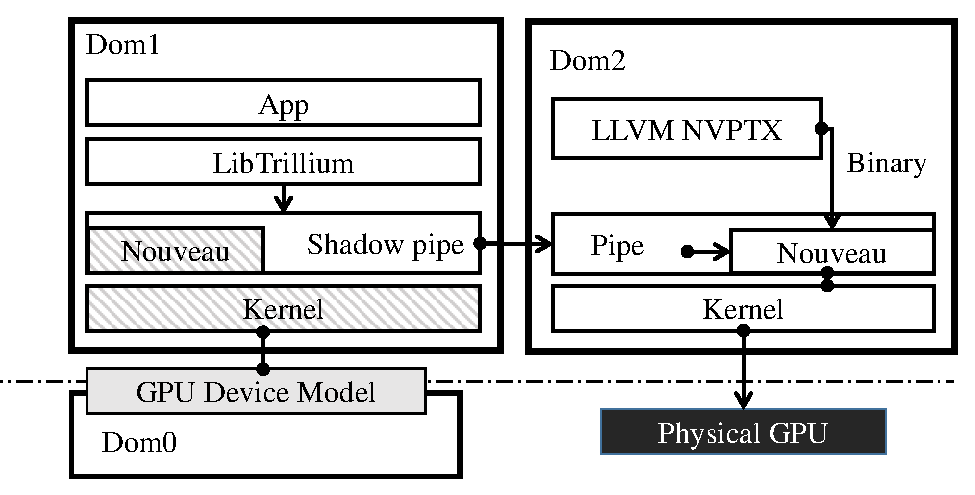
\includegraphics[width=.5\linewidth,trim={0.6cm 0 0 0},clip]{trillium/images/design/trillium.pdf}
		\caption{The design of \Trillium with shadow pipe.}
		\label{fig_trillium_direct2}
\end{figure*}

\section{\iemts: A new analysis framework}

Traditionally, virtualization designs have been taxonomized
according to the core techniques employed (e.g. emulation, full- or
para-virtualization, API remoting, etc.), and evaluated
in a property trade-off space comprising performance,
compatibility, interposition, and isolation. \emph{Isolation} ensures that
mutually distrustful guests cannot access each other's data or harm each
other's performance. \emph{Compatibility}, characterizes how well a design
preserves the freedom of hardware and software components to evolve
independently: e.g. changes in the hypervisor should not force changes to
guest software. Virtualization provides an indirection layer between
logical and physical resources by \emph{interposing} a well-defined interface.
The quality of interposition determines the nature of benefits (e.g. extent of
consolidation) afforded by a virtualized system~\cite{waldspurger12cacm}.

\begin{figure}[!tt]
	\centering
	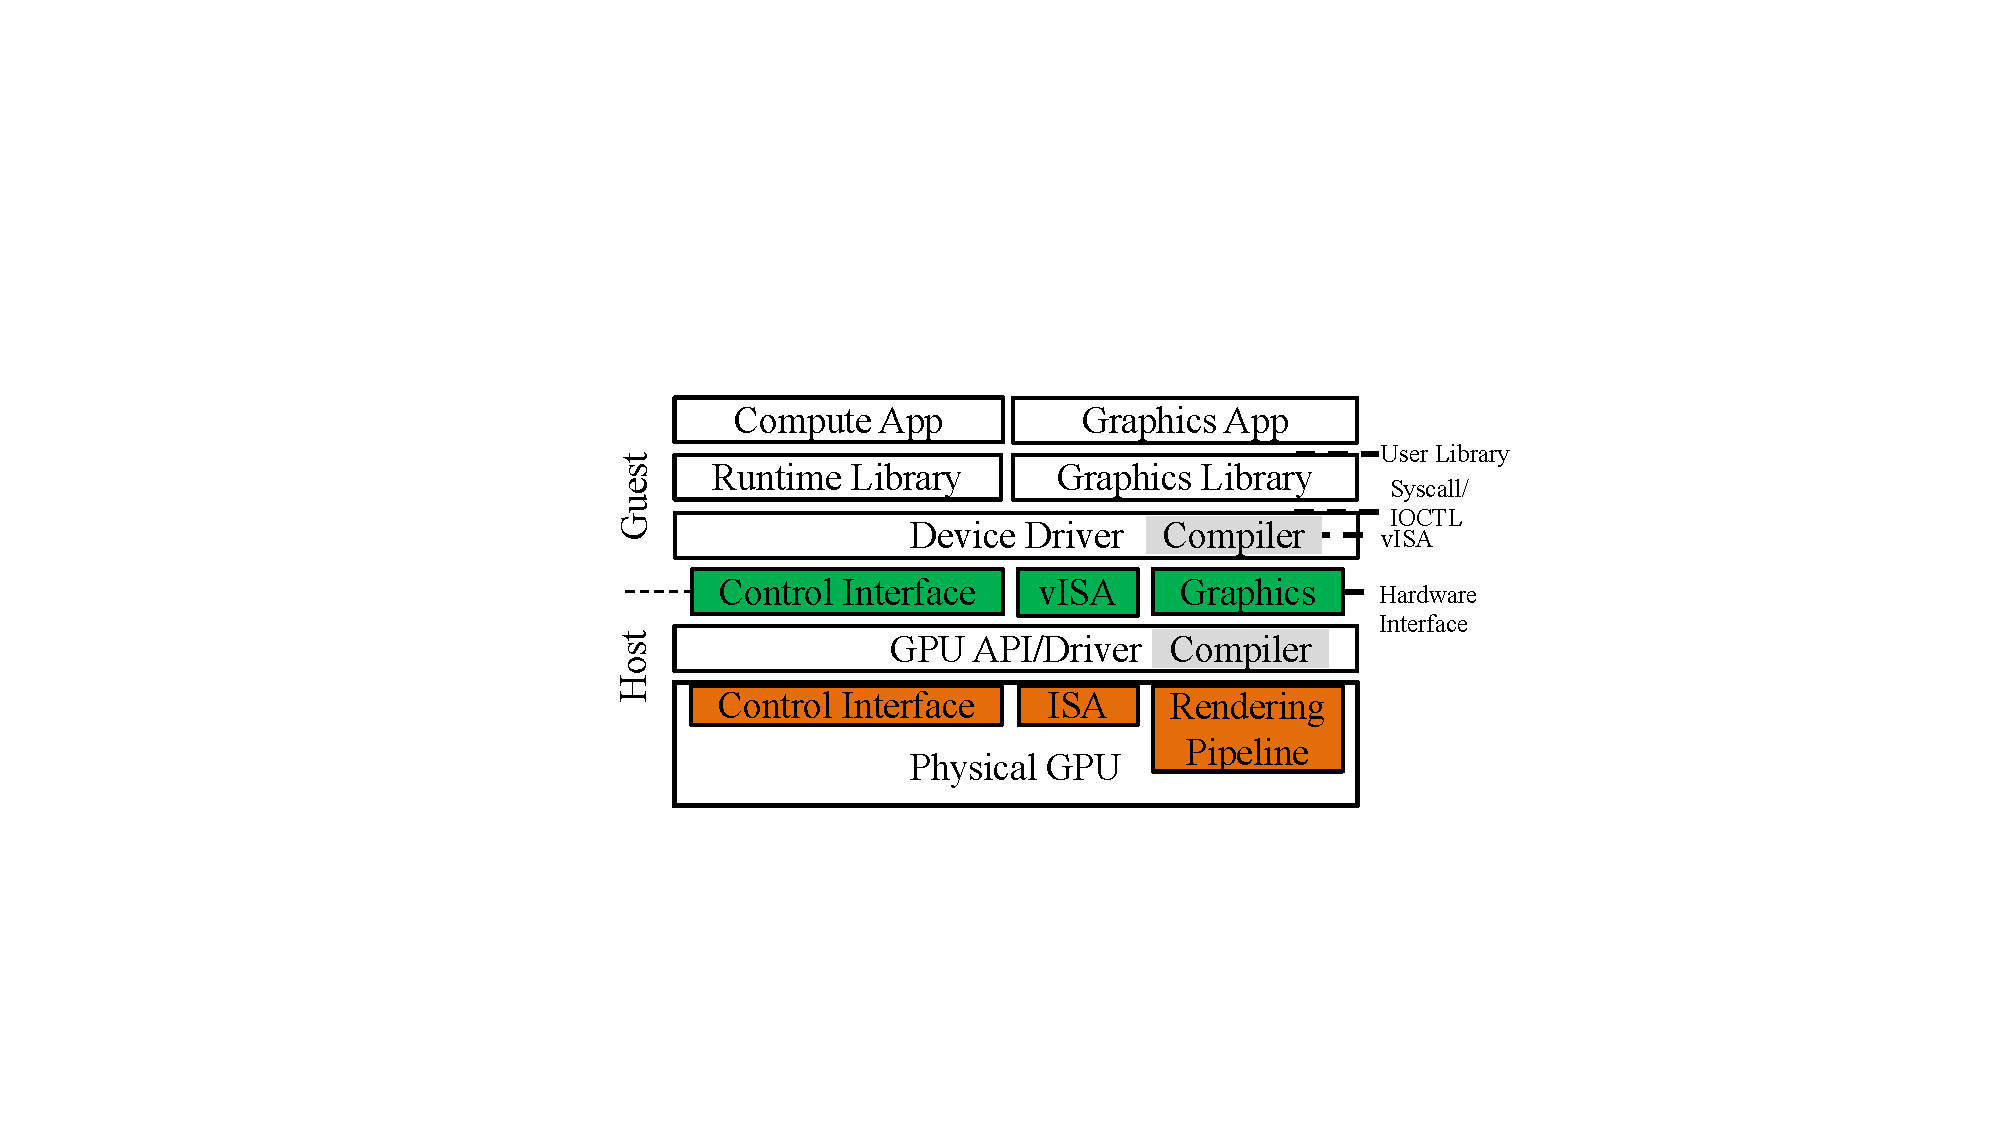
\includegraphics[width=.5\linewidth,trim={10cm 5cm 8cm 6.5cm},clip]{figures/interposition.pdf}
	\caption{Possible points of interposition.}
	\label{fig_interposition}
\end{figure}

A key limiting concern for GPU virtualization is the absence of interposable
interfaces. GPUs are controlled through vendor-specific programming frameworks
(often more than one), key parts of which are often proprietary.Research
to-date on first-class OS abstractions for GPUs~\cite{ptask, dandelion,
silberstein2013gpufs,timegraph, gdev, gpunet} has not impacted practice, and
GPU software stacks actively avoid or bypasss system software. Consequently,
hypervisors are left without clean interfaces to virtualize. Moreover, in
contrast to many other common devices, GPUs have \emph{multiple} interfaces,
such as MMIO and ISA, that may require virtualization.
Figure~\ref{fig_interposition} shows potential interposition points in an GPU
virtualization system: the user-space library, the syscall/ioctl interface
the user-space API operates on, or the hardware interface. Additionally the
GPU's ISA may also be virtualized. Typically, lower layers present finer
granularity of interposition for the hypervisor, but also sacrifice
performance.

We posit that the current \emph{de facto} taxonomy and property trade-off
space are illustrative but not informative for DSAs.
First, Classifying virtualization designs as API-remoting vs. full vs.
para-virtual captures important concepts, and emergent properties compactly,
but doesn't explain their correlation to properties like performance.
Second, virtualization properties such as compatibility, isolation, and
interposition have highly context-dependent meaning and their relative value
to system designers can be hard to quantify.
Consider compatibility: there are many dimensions to compatibility (library,
hardware, OS, etc.), and each of those are commonly achieved by separate
technical, and non-technical means (e.g., TGSI is the common vISA for both the
VMware and GNU/Linux graphics stacks; this is \emph{not a lucky coincidence}).
It is common to see systems compared to other systems intended as exemplars
for a technique or design pattern. Ironically, the end-to-end comparison
presented in the prior chapter on \Trillium is guilty of exactly this: we
compared \Trillium against other systems intended to represent ``full
virtualization'', ''API remoting'', and so on.
Methodologically, such a comparison is laudable: evaluating a design
exhaustively against plausible alternatives in an end-to-end setting is
fundamental to good science. However, its value for drawing out fundamental
insights is scant because ``full virtualization'' only talks about the quality
of the guest-visible abstraction, while findings involving ``API remoting''
are really about the particular API in question. ``Para-virtualization'' is
often cast as a design dimension, ultimately grouping designs that share no
core techniques, such as SVGA and GPUvm. As a framework within which to seek
higher-level insights about design, a rough taxonomy that fails to cleanly
separate most concerns is in unacceptable.

We argue that practical design goals, such as providing a virtualization layer
with specific characteristics, get obscured when these properties are
considered as a set of constraints that must be preserved, without first
refining for context.
Further, production systems, such as VMware SVGA~\cite{dowty2009gpu},
compose multiple virtualization techniques in order to leverage the best
properties of each technique, especially in the presence of multiple
interfaces.

To enable a cleaner separation of concerns, we draw on the observation that
\textit{all} virtualization relies on encapsulation and interposition, and
note that a design can be clearly understood by identifying:
\begin{itemize}[nosep, topsep=0em, leftmargin=1em,labelwidth=*,align=left]
\item the \textbf{I}nterface that is interposed,
\item the \textbf{E}nd-points (source and destination) the interposed event is
transported between,
\item the \textbf{M}echanism used to interpose,
\item the \textbf{T}ransport mechanism used to communicate between endpoints,
\item the mechanisms used to \textbf{S}ynthesize or implement the desired
functionality at the destination. We call this the \textbf{\iemts} framework.
\end{itemize}

\begin{table*}[tt!]
\centering
\footnotesize
\resizebox{\textwidth}{!}{%
\begin{tabular}{@{}p{0.25\linewidth}|p{0.18\linewidth}|p{0.18\linewidth}|p{0.2\linewidth}|p{0.2\linewidth}@{}}
\toprule
\multirow{2}{*}{}         & \multirow{2}{*}{GPUvm} & \multicolumn{2}{c|}{VMware SVGA}         & \multirow{2}{*}{rCUDA} \\
                          &                        & Control Interface  & GPU ABI             &                        \\ \midrule
Interposed Interface      & MMIO/BAR               & DirectX APIs       & Device ISA          & Userspace API          \\
Interposition Source      & Trap handler           & Guest driver/libs  & Guest Driver        & Guest Library          \\
Interposition Destination & Host driver            & Host framework     & Host Driver         & Host/Server Daemon     \\
Interposition Mechanism   & Trap                   & Guest library      & Compilation to vISA & Guest Library Shim     \\
Transport                 & Fault                  & Hypervisor FIFOs   & Hypervisor FIFOs    & RPC                    \\
Synthesis                 & Emulation              & Call host API      & Binary translation  & Call Server API        \\ \bottomrule
\end{tabular}
}
\caption{Comparing virtualization designs using the \texttt{IEMTS} framework.}
\label{tab:new-dims}
\end{table*}

Table~\ref{tab:new-dims} presents analysis of three prior GPU virtualization
systems under the \iemts framework. A quick glance at the table
tells us that GPUvm's~\cite{suzuki2014gpuvm} performance woes arise from its
reliance on trapping and emulating the guest's MMIO accesses. VMware's SVGA
has two entries in the table because there are two interfaces being
virtualized: the control interface (the DirectX/OpenGL API) and the shader ISA.
Explicitly separating the two interfaces helped us realize that
ISA-virtualization is not necessary for accelerator virtualization in the
Trillium project. Further, it became obvious to us that the control interface
virtualization in SVGA and the API-remoting in rCUDA look almost the same
under IEMTS with the exception of the transport. This observation led us
to design AvA's hypervisor-mediated API-remoting scheme, and shift our
attention to solving the compatibility effort via automation.


% ==================

We found that analysing designs using the IEMTS framework facilitated a number
of key insights that should inform future designers of GPGPU virtualization.
Table~\ref{tab:new-dims} illustrates how three prior systems are represented under this framework.
GPUvm\cite{GPUvm}, a full-virtual\-ization research system,
uses costly trap-based interposition.
%modern GPUs rely on communication
%through MMIO/PCIe BARs, leaving few alternatives for interposing between the
%driver and the device.
SVGA~\cite{dowty2009gpu} is a para-virtual device, and thus is free to use any interface for
driver-device communication. It is represented  in the table by two columns, one for
each interface it virtualizes: the control interface and the ISA.
The table clearly illustrates that SVGA uses API-remoting, but other dimensions
enable insight into why the design is attractive despite the compatibility and
interposition conventionally thought be lost by the technique.
While SVGA and rCUDA~\cite{vmCUDA, rCUDA}
% of DirectX graphics libraries
% share a striking and informative similarity:
are both forwarding framework APIs,
they do so over different transports:
SVGA implements the transport layer over hypervisor-managed FIFO queues,
enabling hypervisor interposition that is impossible with the RPC transport used by rCUDA.
SVGA's design mandates modifications to guest libraries and drivers.
However, this lost compatibility is retrieved through non-technical means:
VMware's SVGA driver is integrated into commodity OSes.
VMware also maintains the Linux graphics stack, enabling it to ensure compatibility.

As we observed earlier, the use of para-virtual techniques based on a guest virtual device
is essential for recovering interposition in the absence of clean intermediate stack layers.
The need for that interface to export a full-featured virtual device abstraction
is less evident, especially given the high overheads from having to rely on trap-based
interposition.